\chapter{ARIMA Model}

The goal of this section is to fit log prices and log returns into an autoregressive (AR), moving average (MA), or some combination of the two (ARMA, ARIMA). Figure (\ref{fig:acf_pacf_log_price_returns}) shows the ACF for the log prices (a), PACF of the log prices (b), ACF for the log returns (c) and the PACF for the log returns (d). For AR models, we would expect the ACF to show a gradual decay where the tail cuts off at some point, where the PACF would sharply cut off at lag $p$, then drop to approximately zero. We expect the opposite for MA models, where the ACF significantly cuts off at lag $q$ (then drops off to near zero), and the ACF gradually decays. On the other hand, the ACF and PACF for the ARMA(p,q) model will not clearly indicate where the lags cut off. 

\begin{figure}[h]
	\centering
	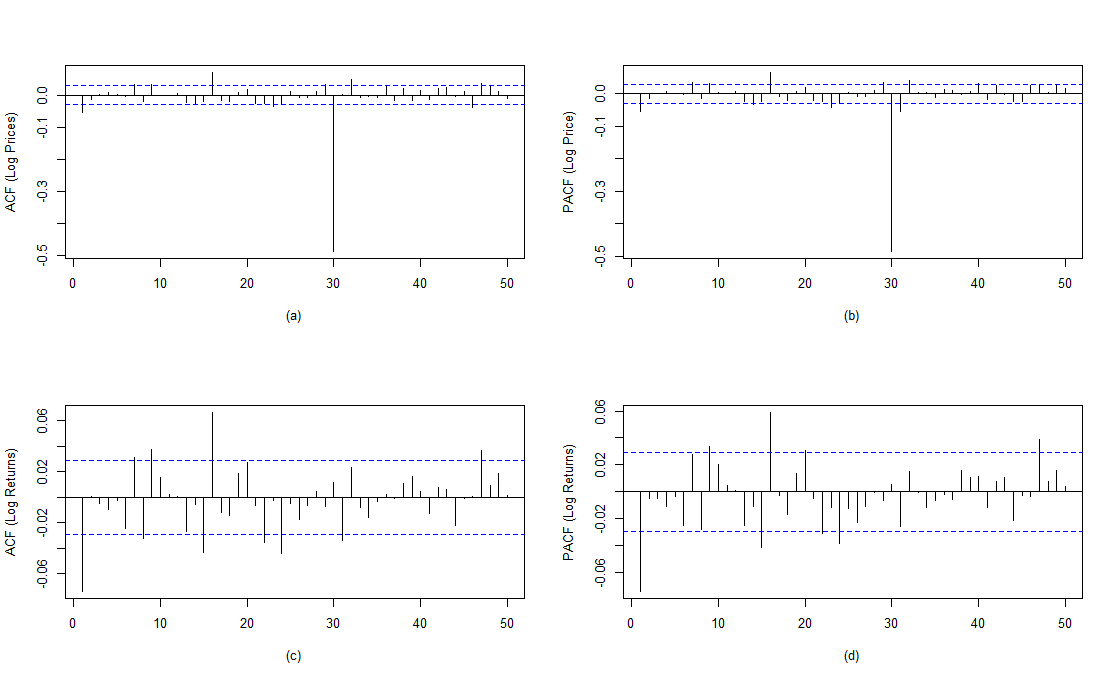
\includegraphics[width=1\linewidth]{content/plots/acf_pacf_log_price_returns.png}
	\caption{ACF and PACF for the log returns/prices of QCOM}
	\label{fig:acf_pacf_log_price_returns}
\end{figure}

We first examine the log prices of QCOM. As we can see from Figure (\ref{fig:acf_pacf_log_price_returns}), the ACF plot (a) for the log prices shows a very sharp spike at lag 0, and a significant lag around point 30; the rest is essentially noise. This plot is not very useful, because the time series is non-stationary. We have the same pattern when looking at the PACF plot (b) for the log prices, as we see mostly noise and a large spike around lag 30. Again, this plot is not very reliable since stationary is required for the PACF/ACF patterns to inform model selection. 

Looking at the ACF plot (c) log returns, we have a slight negative spike at lag 1. We also have a lot of significant lags that show up every 3 or 4 lags. Looking at the PACF plot (d), there are many small spikes, some of which are at lag 5, 8, 15, etc., but none are dominant. There is no clear cut-off in the PACF plot; we also do not see a gradual decline, which is consistent with the MA process. Using this plot, we cannot determine whether or not we should use an MA or AR model. We also consider using ARMA($p,q$) models.

The ARMA model (AutoRegression Moving Average) is a time series model used to describe stationary processes, which combines the past values of the AR($p$) model and the past forecasting errors of the MA($q$) model. We define the model as follows:
\begin{equation}
	r_t=\phi_0+\sum_{i=1}^{p}\phi_ir_{t-i}+a_t-\sum_{i=1}^{q}\theta_ia_{t-i},
\end{equation}
where $\lbrace a_t\rbrace$ is a white noise series and $p$ and $q$ are nonnegative integers. Since the ACF and PACF are not informative in determining the order of an ARMA model, we use the extended autocorrelation function (EACF) to specify the order of an ARMA process. If we have a consistent estimate of the AR component of an ARMA model, we can derive the MA component. From the derived MA series, we can use ACF to identify the order of an MA component.
\begin{table}[H]
	\centering
	\caption{Extended Autocorrelation Function (EACF) for QCOM Log Returns}
	\begin{tabular}{c|cccccccccccccc}
		$(p, q)$ & 0 & 1 & 2 & 3 & 4 & 5 & 6 & 7 & 8 & 9 & 10 & 11 & 12 & 13 \\
		\hline
		0 & x & o & o & o & o & x & x & x & x & o & o & o & o & o \\
		1 & x & o & o & o & o & o & o & o & o & o & o & o & o & o \\
		2 & x & o & o & o & o & o & o & o & o & o & o & o & o & o \\
		3 & x & o & o & o & o & o & o & o & o & o & o & o & o & o \\
		4 & x & x & o & o & o & o & o & o & o & o & o & o & o & o \\
		5 & x & x & x & o & o & o & o & o & o & o & o & o & o & o \\
		6 & x & x & x & x & o & o & o & o & o & o & o & o & o & o \\
		7 & x & x & x & x & x & o & o & o & o & o & o & o & o & o \\
		\label{tab:eacf}
	\end{tabular}
\end{table}
Unlike the standard ACF and PACF -- which are more effective for pure AR or MA models -- the EACF is especially useful when dealing with mixed ARMA models. The output of an EACF is a two-way table, where the rows correspond to AR order $p$ and the columns to MA order $q$. Table (\ref{tab:eacf}) shows the Theoretical EACF for an ARMA model, where X denotes statistically significant autocorrelation, and O denotes statistically insignificant autocorrelation, which suggests a good candidate for the true model. In general, for an ARMA($p,q$) model, the triangle of O will have its upper left vertex at the $(p, q)$ position, which we can see is an ARMA($1,1$) model. This will be the basis for our model selection.
\section{Model Selection}

ARMA(1,1) is the basis for our models, but as we can see from the EACF, we can also consider entries that fall inside the "O triangle" (starting at $p=1,q=1$). The residuals at these points are also insignificant and potentially valid model candidates. Considering this, we also consider ARMA(1, 2), ARMA(2, 1), ARMA(2, 2), ARMA(1, 3), and ARMA(0, 2). We have picked a combination of models that either add an extra AR or MA term to balance our selection criteria. 

Table (\ref{tab:aic}) the selected fit for both the log returns and the log prices. The log prices includes both seasoning and regular differencing. For the selection criteria we use the AIC, which indicates a better-fitting model with a balance between the goodness of fit and model complexity. We choose the model with the smallest AIC, which is the ARMA(2,2) for the log prices and ARMA(0,2) for the log returns.

\begin{table}[ht]
	\centering
	\caption{AIC for Log Prices and Log Returns}
	\begin{tabular}[t]{lccccc}
		\toprule
		&ARMA(1,1)& ARMA(2,1) & ARMA(2,2) & ARMA(1,3) & ARMA(0,2)\\
		\midrule
		Log Prices & -21945.69 & -21943.79 & -21943.32 & -21941.81 & -21945.81  \\				
		Log Returns & -21958.18 & -21956.2 & -21954.39 & -21954.37 & -21958.15 \\				
		\bottomrule
	\end{tabular}\label{tab:aic}
\end{table}

\section{Forecasting}

Like the behavior of ACF, forecast of an ARMA($p,q$) model have similiar characteristics as those of an AR($P$) model after adjusting for the impacts of the MA component. The form for the $\ell$-step-ahead forecast is the following:
\begin{equation}
	\hat{r}_h(\ell)=E(r_{h+\ell}|F_h)=\phi_0+\sum_{i=1}^{p}\phi_i\hat{r}_h(\ell-i)-\sum_{i=1}^{q}\theta_ia_h(\ell-i)
\end{equation}

Figure (\ref{fig:forecast}) presents a 1000-step ahead forecast for both the log prices (left panel) and log returns (right panel) of QCOM based on fitted ARIMA models.

The left panel shows the forecast from an ARIMA(2,1,2)(0,1,0) model applied to the log price series. The forecasted trajectory exhibits a flattening trend with widening confidence intervals over time, reflecting increasing uncertainty as the forecast horizon extends. Despite recent upward momentum in the log price, the model projects a relatively stationary mean path, suggesting that much of the recent trend may not persist in the long term. The fan-shaped prediction intervals highlight the stochastic nature of the process, primarily due to the seasonal and regular differencing applied.

\begin{figure}[h]
	\centering
	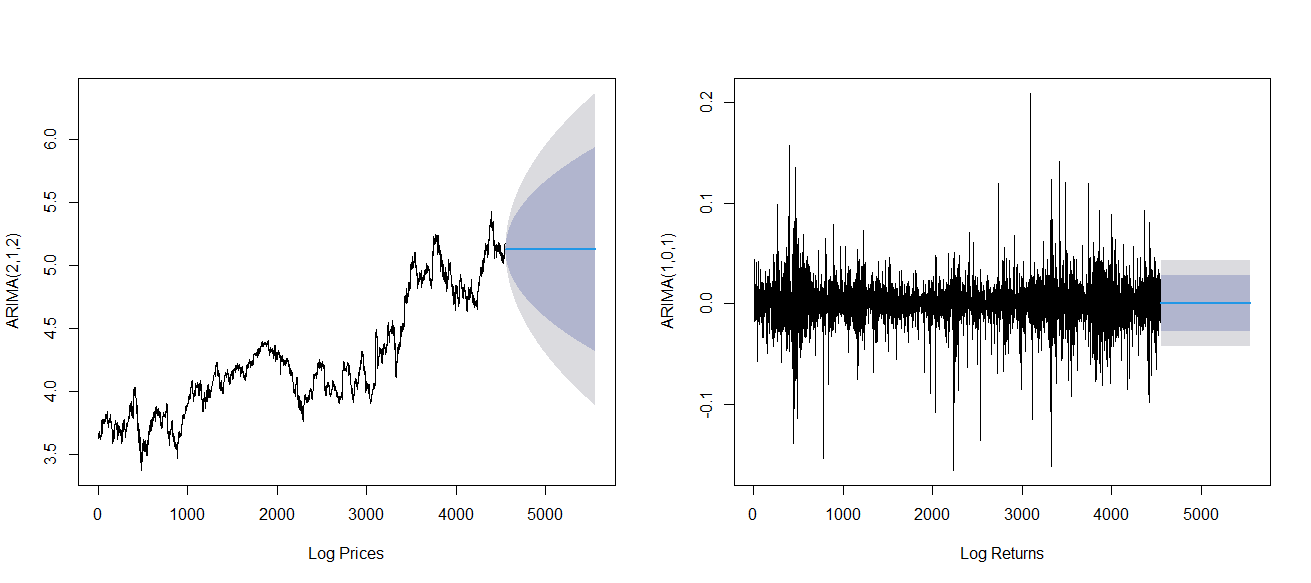
\includegraphics[width=1\linewidth]{content/plots/forecast.png}
	\caption{1000 Step Ahead Forecast for the Log Returns and Prices}
	\label{fig:forecast}
\end{figure}

Figure (\ref{fig:residual_plot_212}) shows the residual diagnostics for the fitted ARIMA(2,1,2) model applied to the QCOM log returns. The right panel displays the forecast from an ARIMA(0,1,1) model fitted to the log returns. The forecasted returns converge quickly to a mean close to zero, with narrow and stable confidence bands. This behavior aligns with the efficient market hypothesis, where log returns are assumed to be white noise, and thus, future returns are unpredictable based on past behavior. The low variance and flat mean reinforce the conclusion that the return process is stationary and lacks significant autocorrelation beyond short lags.

The right panel displays the forecast from an ARIMA(0,1,1) model fitted to the log returns. The forecasted returns converge quickly to a mean close to zero, with narrow and stable confidence bands. This behavior aligns with the efficient market hypothesis, where log returns are assumed to be white noise, and thus, future returns are unpredictable based on past behavior. The low variance and flat mean reinforce the conclusion that the return process is stationary and lacks significant autocorrelation beyond short lags.

Overall, the forecast results suggest that while log prices show medium-term variability and are influenced by both trend and seasonal components, the log returns remain largely mean-reverting with no significant drift, supporting the appropriateness of ARIMA models in modeling these two distinct dynamics.
\begin{figure}[h]
	\centering
	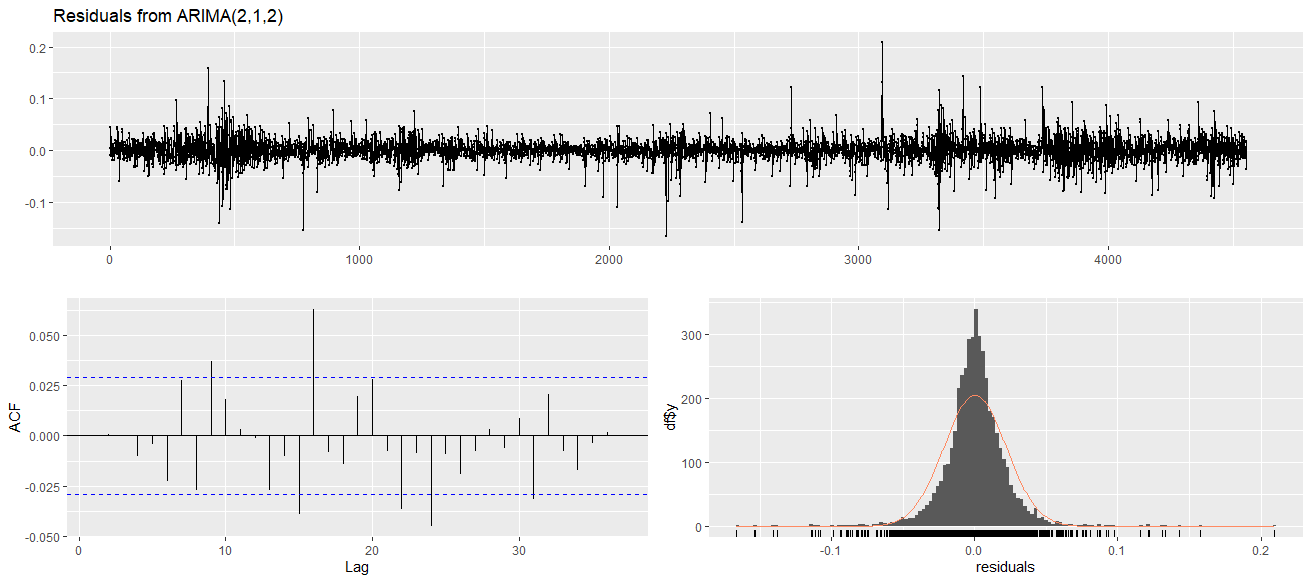
\includegraphics[width=1\linewidth]{content/plots/residual_plot_212.png}
	\caption{Residual Plots for the ARIMA(2,1,2) model for the Log Returns}
	\label{fig:residual_plot_212}
\end{figure}
The top panel shows the standardized residuals over time. The residuals appear to fluctuate around zero with no visible trend or systematic pattern, suggesting that the model has effectively captured the underlying structure of the time series. Some sporadic large residuals are observed, but they are infrequent and do not persist.

The bottom-left panel shows the ACF of the residuals, where most autocorrelations lie well within the 95\% confidence boundary. This indicates the absence of significant autocorrelation in the residuals, confirming that the ARIMA model has adequately removed time dependence from the series.

The bottom-right panel shows a histogram of the residuals overlaid with a normal density curve. The residuals are approximately centered at zero and exhibit a roughly bell-shaped distribution, although there is some evidence of slight fat tails compared to a normal distribution.

Overall, the diagnostic plots support the adequacy of the ARIMA(2,1,2) model. The residuals behave like white noise — they are uncorrelated and approximately normally distributed — suggesting that the model is a good fit for the data and suitable for forecasting purposes. Figure (\ref{fig:residual_plot_1_1}) also exhibits the same residual distribution for the ARIMA(1,0,1) model with the log prices.